% !TEX root = ../main.tex
% chktex-file 46
\chapter{Einleitung}%
\label{sec:intro}

\pagenumbering{arabic}			% arabic page numbering
\setcounter{page}{1}			% set page counter

\cleanchapterquote{
The actual world cannot be distinguished from a world of imagination by any description.
Hence the need of pronoun and indices, and the more complicated the subject the greater the need of them.
}{Charles Sanders Peirce}{Mathematiker und Philosoph}

\section{Motivation}%
\label{sec:intro:motivation}

In den letzten Jahren hat die Repräsentation von Wissensbasen durch Graphen, sog. Wissensgraphen, immer mehr an Bedeutung gewonnen.
Google, Bing und IBM Watson benutzen solche Wissensgraphen z.~B. zum Beantworten von komplexen Suchanfragen.

Die Grundidee dabei ist es, Entitäten durch Knoten und Relationen durch Kanten abzubilden.
Entitäten können konkrete Dinge, wie z.~B. Personen, aber auch abstrakte Konzepte, wie z.~B. historische Epochen, sein.
Relationen beschreiben beliebige Beziehungen zwischen den Entitäten, z.~B. $person(\text{Da~Vinci}) \xrightarrow{\text{lived~in}} epoch(\text{Renaissance})$.
Die Entität, von der eine solche Relation ausgeht, wird als Subjekt und die Zielentität als Objekt der Relation bezeichnet.

Die Arten von Entitäten bzw.\ Relationen (z.~B. $person$ bzw. $lived~in$) und deren Bedeutung sind dabei i.~d.~R. formal in einer sog.\ Ontologie spezifiziert.
Die Ontologie beschränkt also die Menge gültiger Wissensgraphen, was eine effiziente maschinelle Verarbeitung der im Graph enthaltenen Informationen ermöglicht.

Da Wissensgraphen in zahlreichen Domänen einsetzbar sind, wird deren automatisierte Konstruktion bereits seit Jahren erforscht.
Manuelles Konstruieren und vor allem anschließendes Warten und Aktualisieren von Wissensgraphen ist aufgrund der abzubildenden Datenmengen nicht praktikabel.
Bei einer maschinellen Konstruktion sind insbesondere zwei Anforderungen problematisch:
\begin{enumerate}
	\item Das Verarbeiten von unstrukturierten Eingaben, wie z.~B. natürlichsprachlichen Texten.
	\item Effizientes Eingliedern neuer Informationen in einen bestehenden Wissensgraphen.
		Dieses Eingliedern von Informationen umfasst insbesondere:
		\begin{itemize}
			\item \textbf{Entity Resolution:}
				Hinzukommende Entitäten, die bereits im Graphen enthalten sind, müssen als Duplikate erkannt werden.
				Dies ist i.~d.~R. nicht trivial, da dieselbe Entität durch viele verschiedene, oftmals vom Kontext abhängige Token repräsentiert werden kann;
				z.~B. \textit{Bob} vs. \textit{Robert} oder \textit{Papst} vs. \textit{Franziskus}.
			\item \textbf{Link Prediction:}
				Hinzukommende Entitäten müssen mit bereits bestehenden Entitäten in Relation gesetzt werden.
				Hinzukommende Relationen können zudem benutzt werden um andere Relationen zu inferieren;
				z.~B. \[\mathit{female}(A) \land B \xrightarrow{\text{son~of}} A \implies A \xrightarrow{\text{mother~of}} B\]
		\end{itemize}
\end{enumerate}

Die Kombination dieser beiden Anforderungen ist interessant, da das meiste verfügbare Wissen in natürlichsprachlicher Textform vorliegt und zudem permanent neues Wissen entsteht.
Ein automatisiertes Wissensgraph-Konstruktionsverfahren, welches beide Anforderungen berücksichtigt, ist daher in diversen Domänen von Nutzen.
Ein Beispiel hierfür ist die Auswertung von Kommunikationsdaten aus E-Mails oder Chat-Nachrichten mit dem Ziel die sozialen Beziehungen und Intentionen der Kommunikationpartner zu ermitteln.

\section{Ziele der Arbeit}%
\label{sec:intro:goals}

Das übergeordnete Ziel dieser Arbeit ist es, ein Verfahren zu finden, welches das soeben beschriebene Problem der automatisierten Wissensgraph-Konstruktion für Kommunikationsdaten löst.
Konkret sei ein Stream von Textnachrichten, wie z.~B.\ E-Mails, gegeben, denen jeweils ein Inhalt, ein Absender, ein Empfänger und ggf.\ weitere Metadaten, wie z.~B. die Absendezeit, zugeordnet ist.
Die Nachrichteninhalte werden der Einfachheit halber als ausschließlich englischsprachig angenommen.
Außerdem wird eine --- für E-Mails und andere Kurznachrichten typische --- eingeschränkte Sprachkomplexität angenommen.
Die Nachrichten sollen nacheinander in das zu konstruierende System eingefügt werden, welches sukzessive einen Wissensgraphen daraus erzeugt.

Für diese Erzeugung müssen im Wesentlichen drei Teilprobleme gelöst werden:
\begin{enumerate}
	\item \textbf{Onotologie:}
		Spezifikation einer Ontologie für die Domäne des Wissensgraphen, die mächtig genug ist, um möglichst diverse natürlichsprachlich beschriebene Informationen abzubilden.
		Im Folgenden wird diese Ontologie Wissensgraphontologie genannt.
	\item \textbf{Sprachverarbeitung:}
		Konzeption eines Verfahrens, welches die natürlichsprachlichen Inhalte der Nachrichten in eine für die Wissensgraph-Konstruktion geeignete Form bringt.
	\item \textbf{Grapherweiterung:}
		Konzeption eines Verfahrens, um eine eintreffende Nachricht in den bestehenden Wissensgraphen einzufügen.
\end{enumerate}
Die Teillösungen können zu einem Konstruktionsverfahren kombiniert werden, welches grob wie folgt aufgebaut ist:
\begin{figure}[h]
	\centering
	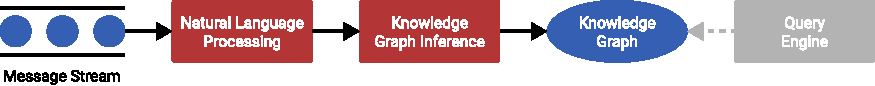
\includegraphics[width=0.82\textwidth]{gfx/introduction/overview.pdf}
	\caption{Grober Aufbau des Konstruktionsverfahrens}\label{fig:intro:overview}
\end{figure} \\
Mittels eines Verfahrens zur Sprachverarbeitung und Grapherweiterung wird ein Wissensgraph konstruiert, der die spezifizierte Ontologie benutzt.
Der Zweck dieses Wissensgraphen ist, dass er mittels eines Anfragesystems ausgelesen werden kann und so zur Beantwortung von Fragen über den Inhalt der eingegebenen Nachrichten benutzt werden kann.
Die Aufgabenstellung dieser Arbeit beschränkt sich allerdings auf die Konstruktion, der Aufbau eines Anfragesystems wird nicht beschrieben.

Das gemäß \figreft{fig:intro:overview} zusammengesetzte Verfahren muss folgende technische Anforderungen erfüllen:
\begin{enumerate}
	\item \textbf{Erweiterbarkeit:}
		Es soll prinzipiell möglich sein, zusätzlich zur Sprachverarbeitung auch andere Verarbeitungsverfahren, z.~B. für Bilder, hinzufügen zu können.
		Insbesondere die Graphontologie darf also nicht zu sehr auf die Struktur natürlicher Sprache zugeschnitten sein, damit auch Informationen aus nicht natürlichsprachlichen Datenquellen repräsentierbar sind.
	\item \textbf{Parallelisierbarkeit:}
		Das Verfahren soll in der Lage sein, die Rechenleistung mehrerer Prozessorkerne bzw.\ Prozessoren zu nutzen.
		Diese Anforderung betrifft insbesondere das Grapherweiterungsverfahren.
\end{enumerate}

Diese Arbeit entstand in Kooperation mit der Firma Atos.
Die soeben beschriebenen Ziele und technischen Anforderungen waren dabei vorgegeben.
Eine weitere Anforderung war die prototypische Implementation des entwickelten Verfahrens.
Ziel ist es dabei jedoch nicht, eine Software zu entwickeln, welche sich in der Praxis einsetzen lässt.
Vielmehr geht es darum, prototypisch aufzuzeigen, wie die Wissensgraph-Konstruktion aus Kommunikationsdaten prinzipiell ablaufen kann.

\section{Aufbau der Arbeit}%
\label{sec:intro:structure}

Die drei Komponenten Ontologie, Sprachverarbeitung und Grapherweiterung bilden die Basis des zu entwickelnden Systems und gliedern daher auch diese Arbeit.
In den Kapiteln~\ref{sec:related} bis~\ref{sec:text2kg} werden diese Komponenten schrittweise genauer betrachtet, was am Ende in einem konkreten Verfahren zur Wissensgraph-Konstruktion resultiert.

\paragraph{Kapitel~\ref{sec:related}: \nameref{sec:related}}
Im ersten Schritt wird ein Überblick über die bisherige Forschung und vorhandenen Technologien gegeben.
Das Finden einer Graphontologie lässt sich als ein Problem der Wissensrepräsentation verstehen, daher wird zuerst ein Überblick über die bisherige Entwicklung von Wissensrepräsentationsverfahren gegeben.
Anschließend folgt ein Überblick über verbreitete Werkzeuge zur Sprachverarbeitung.
Zuletzt wird beschrieben, welche Ansätze es zur Konstruktion von Wissensgraphen mit einer gegebenen Ontologie aus gegebenen Eingabedaten gibt.

\paragraph{Kapitel~\ref{sec:theory}: \nameref{sec:theory}}
Da diese Arbeit direkt auf manchen der in Kapitel~\ref{sec:related} vorgestellten Arbeiten aufbaut, werden diese Arbeiten hier näher erläutert.
Zuerst werden die sog.\ Konzeptgraphen beschrieben, da die verwendete Graphontologie auf ihnen aufbaut.
Es folgt ein Überblick über den Aufbau von CoreNLP, dem verwendeten Werkzeug zur Sprachverarbeitung.
Zuletzt wird eine kurze Einführung in HL-MRFs gegeben, eine Klasse von graphischen Modellen, welche zur Konstruktion von Wissensgraphen benutzt werden kann.

\paragraph{Kapitel~\ref{sec:text2kg}: \nameref{sec:text2kg}}
Basierend auf den in Kapitel~\ref{sec:theory} vorgestellten Arbeiten wird nun die konkret verwendete Ontologie, das Sprachverarbeitungsverfahren und die Grapherweiterung beschrieben.
Außerdem wird kurz erläutert, wie das resultierende Gesamtverfahren implementiert wurde.

\paragraph{Kapitel~\ref{sec:evaluation}: \nameref{sec:evaluation}}
Um die Stärken und Schwächen des in Kapitel~\ref{sec:text2kg} beschriebenen Verfahrens aufzuzeigen, wird es hier mit realen Kommunikationsdaten getestet.
Da es bislang keine Testdatensets gibt, die gut für die Evaluation des entwickelten Verfahrens geeignet sind, erfolgen keine umfangreichen empirischen Tests.
Stattdessen wird stichprobenartig ein kleines Nachrichten-Set eingefügt.
Der resultierende Wissensgraph wird anschließend manuell untersucht.

\paragraph{Kapitel~\ref{sec:conclusion}: \nameref{sec:conclusion}}
Abschließend werden die Ergebnisse zusammengefasst und ein Ausblick auf Möglichkeiten der Weiterentwicklung des Systems gegeben.
